\subsection{Keypoint Detection and Feature Description}

Extracting information from images is a common task in computer vision.
One approach is the detection of salient regions of special interest --- \emph{features}.
Such regions can have arbitrary detectable properties, like a sharp brightness gradient or being corner-like.
Detecting such a region results in a \emph{keypoint} that might have properties like a \emph{size}, \emph{response} and sometimes even an \emph{orientation} (Figure~\ref{fig:features_example}).
\begin{figure}[H]
    \scalebox{0.95}{%
    

\tikzset{every picture/.style={line width=0.75pt}} %set default line width to 0.75pt        

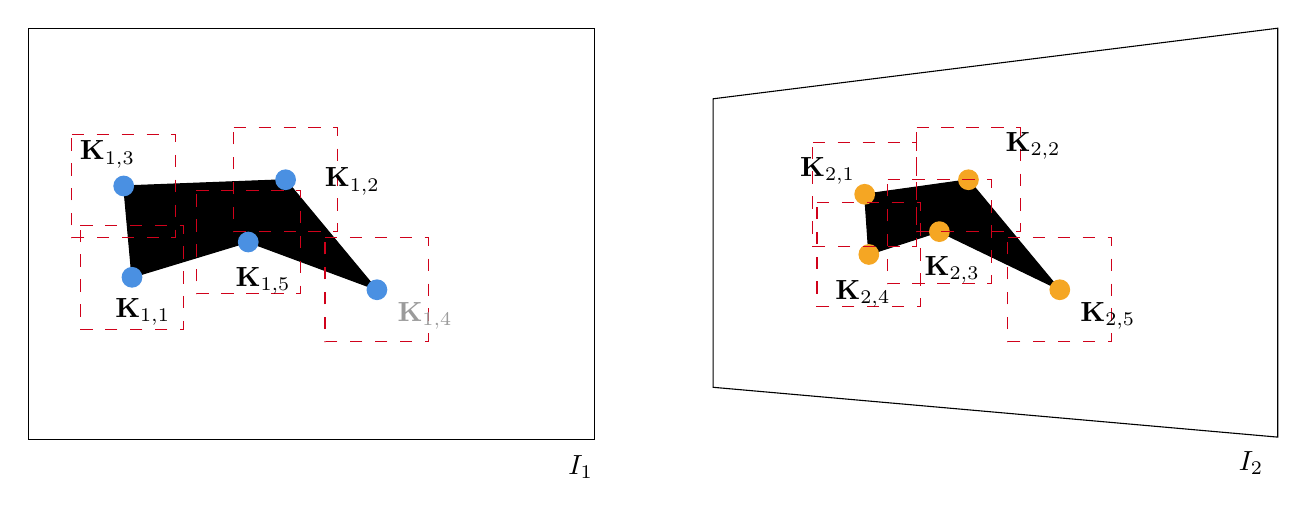
\begin{tikzpicture}[x=0.75pt,y=0.75pt,yscale=-1,xscale=1]
%uncomment if require: \path (0,241); %set diagram left start at 0, and has height of 241

%Shape: Rectangle [id:dp035829742459278835] 
\draw   (10,9.33) -- (283,9.33) -- (283,207.33) -- (10,207.33) -- cycle ;
%Shape: Polygon [id:ds9920063897845183] 
\draw  [fill={rgb, 255:red, 0; green, 0; blue, 0 }  ,fill opacity=1 ] (134,82.33) -- (178,135.33) -- (116,112.33) -- (60,129.33) -- (56,85.33) -- cycle ;
%Shape: Circle [id:dp761043588130765] 
\draw  [draw opacity=0][fill={rgb, 255:red, 74; green, 144; blue, 226 }  ,fill opacity=1 ] (173,135.33) .. controls (173,132.57) and (175.24,130.33) .. (178,130.33) .. controls (180.76,130.33) and (183,132.57) .. (183,135.33) .. controls (183,138.09) and (180.76,140.33) .. (178,140.33) .. controls (175.24,140.33) and (173,138.09) .. (173,135.33) -- cycle ;
%Shape: Circle [id:dp13055646965010093] 
\draw  [draw opacity=0][fill={rgb, 255:red, 74; green, 144; blue, 226 }  ,fill opacity=1 ] (129,82.33) .. controls (129,79.57) and (131.24,77.33) .. (134,77.33) .. controls (136.76,77.33) and (139,79.57) .. (139,82.33) .. controls (139,85.09) and (136.76,87.33) .. (134,87.33) .. controls (131.24,87.33) and (129,85.09) .. (129,82.33) -- cycle ;
%Shape: Circle [id:dp8680057373610014] 
\draw  [draw opacity=0][fill={rgb, 255:red, 74; green, 144; blue, 226 }  ,fill opacity=1 ] (111,112.33) .. controls (111,109.57) and (113.24,107.33) .. (116,107.33) .. controls (118.76,107.33) and (121,109.57) .. (121,112.33) .. controls (121,115.09) and (118.76,117.33) .. (116,117.33) .. controls (113.24,117.33) and (111,115.09) .. (111,112.33) -- cycle ;
%Shape: Circle [id:dp7411102135218419] 
\draw  [draw opacity=0][fill={rgb, 255:red, 74; green, 144; blue, 226 }  ,fill opacity=1 ] (55,129.33) .. controls (55,126.57) and (57.24,124.33) .. (60,124.33) .. controls (62.76,124.33) and (65,126.57) .. (65,129.33) .. controls (65,132.09) and (62.76,134.33) .. (60,134.33) .. controls (57.24,134.33) and (55,132.09) .. (55,129.33) -- cycle ;
%Shape: Circle [id:dp2075524582431375] 
\draw  [draw opacity=0][fill={rgb, 255:red, 74; green, 144; blue, 226 }  ,fill opacity=1 ] (51,85.33) .. controls (51,82.57) and (53.24,80.33) .. (56,80.33) .. controls (58.76,80.33) and (61,82.57) .. (61,85.33) .. controls (61,88.09) and (58.76,90.33) .. (56,90.33) .. controls (53.24,90.33) and (51,88.09) .. (51,85.33) -- cycle ;
%Shape: Polygon [id:ds2941998606572992] 
\draw  [fill={rgb, 255:red, 0; green, 0; blue, 0 }  ,fill opacity=1 ] (463,82.33) -- (507,135.33) -- (449,107.33) -- (415,118.33) -- (413,89.33) -- cycle ;
%Shape: Circle [id:dp23309094023669752] 
\draw  [draw opacity=0][fill={rgb, 255:red, 245; green, 166; blue, 35 }  ,fill opacity=1 ] (502,135.33) .. controls (502,132.57) and (504.24,130.33) .. (507,130.33) .. controls (509.76,130.33) and (512,132.57) .. (512,135.33) .. controls (512,138.09) and (509.76,140.33) .. (507,140.33) .. controls (504.24,140.33) and (502,138.09) .. (502,135.33) -- cycle ;
%Shape: Circle [id:dp6238978047230974] 
\draw  [draw opacity=0][fill={rgb, 255:red, 245; green, 166; blue, 35 }  ,fill opacity=1 ] (458,82.33) .. controls (458,79.57) and (460.24,77.33) .. (463,77.33) .. controls (465.76,77.33) and (468,79.57) .. (468,82.33) .. controls (468,85.09) and (465.76,87.33) .. (463,87.33) .. controls (460.24,87.33) and (458,85.09) .. (458,82.33) -- cycle ;
%Shape: Circle [id:dp6090832055278774] 
\draw  [draw opacity=0][fill={rgb, 255:red, 245; green, 166; blue, 35 }  ,fill opacity=1 ] (444,107.33) .. controls (444,104.57) and (446.24,102.33) .. (449,102.33) .. controls (451.76,102.33) and (454,104.57) .. (454,107.33) .. controls (454,110.09) and (451.76,112.33) .. (449,112.33) .. controls (446.24,112.33) and (444,110.09) .. (444,107.33) -- cycle ;
%Shape: Circle [id:dp846464460393933] 
\draw  [draw opacity=0][fill={rgb, 255:red, 245; green, 166; blue, 35 }  ,fill opacity=1 ] (410,118.33) .. controls (410,115.57) and (412.24,113.33) .. (415,113.33) .. controls (417.76,113.33) and (420,115.57) .. (420,118.33) .. controls (420,121.09) and (417.76,123.33) .. (415,123.33) .. controls (412.24,123.33) and (410,121.09) .. (410,118.33) -- cycle ;
%Shape: Circle [id:dp4845841454073171] 
\draw  [draw opacity=0][fill={rgb, 255:red, 245; green, 166; blue, 35 }  ,fill opacity=1 ] (408,89.33) .. controls (408,86.57) and (410.24,84.33) .. (413,84.33) .. controls (415.76,84.33) and (418,86.57) .. (418,89.33) .. controls (418,92.09) and (415.76,94.33) .. (413,94.33) .. controls (410.24,94.33) and (408,92.09) .. (408,89.33) -- cycle ;
%Shape: Polygon [id:ds0993695896079676] 
\draw   (340,43.33) -- (612,9.33) -- (612,206.33) -- (340,182.33) -- cycle ;
%Shape: Square [id:dp8236130174233348] 
\draw  [color={rgb, 255:red, 208; green, 2; blue, 27 }  ,draw opacity=1 ][dash pattern={on 4.5pt off 4.5pt}] (153,110.33) -- (203,110.33) -- (203,160.33) -- (153,160.33) -- cycle ;
%Shape: Square [id:dp6761472971368142] 
\draw  [color={rgb, 255:red, 208; green, 2; blue, 27 }  ,draw opacity=1 ][dash pattern={on 4.5pt off 4.5pt}] (109,57.33) -- (159,57.33) -- (159,107.33) -- (109,107.33) -- cycle ;
%Shape: Square [id:dp06523745964376726] 
\draw  [color={rgb, 255:red, 208; green, 2; blue, 27 }  ,draw opacity=1 ][dash pattern={on 4.5pt off 4.5pt}] (31,60.33) -- (81,60.33) -- (81,110.33) -- (31,110.33) -- cycle ;
%Shape: Square [id:dp3887475640832124] 
\draw  [color={rgb, 255:red, 208; green, 2; blue, 27 }  ,draw opacity=1 ][dash pattern={on 4.5pt off 4.5pt}] (91,87.33) -- (141,87.33) -- (141,137.33) -- (91,137.33) -- cycle ;
%Shape: Square [id:dp6775183704136505] 
\draw  [color={rgb, 255:red, 208; green, 2; blue, 27 }  ,draw opacity=1 ][dash pattern={on 4.5pt off 4.5pt}] (35,104.33) -- (85,104.33) -- (85,154.33) -- (35,154.33) -- cycle ;
%Shape: Square [id:dp0686549638078735] 
\draw  [color={rgb, 255:red, 208; green, 2; blue, 27 }  ,draw opacity=1 ][dash pattern={on 4.5pt off 4.5pt}] (388,64.33) -- (438,64.33) -- (438,114.33) -- (388,114.33) -- cycle ;
%Shape: Square [id:dp20553871041489524] 
\draw  [color={rgb, 255:red, 208; green, 2; blue, 27 }  ,draw opacity=1 ][dash pattern={on 4.5pt off 4.5pt}] (438,57.33) -- (488,57.33) -- (488,107.33) -- (438,107.33) -- cycle ;
%Shape: Square [id:dp9372102954632048] 
\draw  [color={rgb, 255:red, 208; green, 2; blue, 27 }  ,draw opacity=1 ][dash pattern={on 4.5pt off 4.5pt}] (482,110.33) -- (532,110.33) -- (532,160.33) -- (482,160.33) -- cycle ;
%Shape: Square [id:dp5089024455920732] 
\draw  [color={rgb, 255:red, 208; green, 2; blue, 27 }  ,draw opacity=1 ][dash pattern={on 4.5pt off 4.5pt}] (390,93.33) -- (440,93.33) -- (440,143.33) -- (390,143.33) -- cycle ;
%Shape: Square [id:dp7886399279303968] 
\draw  [color={rgb, 255:red, 208; green, 2; blue, 27 }  ,draw opacity=1 ][dash pattern={on 4.5pt off 4.5pt}] (424,82.33) -- (474,82.33) -- (474,132.33) -- (424,132.33) -- cycle ;

% Text Node
\draw (269,214) node [anchor=north west][inner sep=0.75pt]   [align=left] {$\displaystyle I_{1}$};
% Text Node
\draw (592,212) node [anchor=north west][inner sep=0.75pt]   [align=left] {$\displaystyle I_{2}$};
% Text Node
\draw (44,136.33) node [anchor=north west][inner sep=0.75pt]   [align=left] {$\displaystyle  \begin{array}{{>{\displaystyle}l}}
\mathbf{K}_{1,1}\\
\end{array}$};
% Text Node
\draw (145,73.33) node [anchor=north west][inner sep=0.75pt]   [align=left] {$\displaystyle  \begin{array}{{>{\displaystyle}l}}
\mathbf{K}_{1,2}\\
\end{array}$};
% Text Node
\draw (27,60.33) node [anchor=north west][inner sep=0.75pt]   [align=left] {$\displaystyle  \begin{array}{{>{\displaystyle}l}}
\mathbf{K}_{1,3}\\
\end{array}$};
% Text Node
\draw (180,138.33) node [anchor=north west][inner sep=0.75pt]  [color={rgb, 255:red, 155; green, 155; blue, 155 }  ,opacity=1 ] [align=left] {$\displaystyle  \begin{array}{{>{\displaystyle}l}}
\mathbf{K}_{1,4}\\
\end{array}$};
% Text Node
\draw (102,121.33) node [anchor=north west][inner sep=0.75pt]   [align=left] {$\displaystyle  \begin{array}{{>{\displaystyle}l}}
\mathbf{K}_{1,5}\\
\end{array}$};
% Text Node
\draw (391,127.33) node [anchor=north west][inner sep=0.75pt]   [align=left] {$\displaystyle  \begin{array}{{>{\displaystyle}l}}
\mathbf{K}_{2,4}\\
\end{array}$};
% Text Node
\draw (473,56.33) node [anchor=north west][inner sep=0.75pt]   [align=left] {$\displaystyle  \begin{array}{{>{\displaystyle}l}}
\mathbf{K}_{2,2}\\
\end{array}$};
% Text Node
\draw (434,115.83) node [anchor=north west][inner sep=0.75pt]   [align=left] {$\displaystyle  \begin{array}{{>{\displaystyle}l}}
\mathbf{K}_{2,3}\\
\end{array}$};
% Text Node
\draw (374,68.33) node [anchor=north west][inner sep=0.75pt]   [align=left] {$\displaystyle  \begin{array}{{>{\displaystyle}l}}
\mathbf{K}_{2,1}\\
\end{array}$};
% Text Node
\draw (509,138.33) node [anchor=north west][inner sep=0.75pt]   [align=left] {$\displaystyle  \begin{array}{{>{\displaystyle}l}}
\mathbf{K}_{2,5}\\
\end{array}$};


\end{tikzpicture}


    }
    \caption[Schematic feature detection and matching]{\emph{Schematic feature detection and matching.} This figure displays two polygons from different view points. The feature detection algorithm detects the corners of the polygon as keypoints in both images. The order of detection is not stable and establishing the correspondence between the detected keypoints requires further processing. A feature descriptor examines to local neighbourhood of each keypoint, visualized with the red dotted square. This descriptor is then used to find the most similar region around a keypoint of the other image. This process is called \emph{feature matching}.}\label{fig:features_example}
\end{figure}
Keypoints on itself are not descriptive enough to be identified in different images.
A changing view point or even a different camera result in changes to the overall shape and appearance of the scene.
Reliable keypoint identification requires the analysis of bigger image patches.
The \emph{keypoint descriptor} analyzes a predefined region around the centered keypoint and extracts a vector for that region.
Different aspects can be analyzed and Section~\ref{sec:feature_algorithms} introduces the most common algorithms for that task.
The extracted vector has a high dimension with tens to hundreds of elements.

Connecting the keypoints between different images uses the extracted descriptors for each keypoint.
\emph{Similar} descriptors are associated.
Similarity of the descriptors is calculated with a matching norm depdendent on the structure of the descriptor.
Dense real descriptors commonly use the Euclidean norm where as binary descriptors use the hamming norm.
Additional constraints, like geometric consistency, improve the accuracy of the matching result.
For the provided example this result might be
\begin{align*}
    \mathbf{K_{1,2}} &\leftrightarrow \mathbf{K_{2,2}}~\textcolor{darkgreen}{\bullet} &
    \mathbf{K_{1,4}} &\leftrightarrow \mathbf{K_{2,5}}~\textcolor{darkgreen}{\bullet} &
    \mathbf{K_{1,5}} &\leftrightarrow \mathbf{K_{2,3}}~\textcolor{darkgreen}{\bullet} \\
    \mathbf{K_{1,3}} &\leftrightarrow \mathbf{K_{2,4}} &
    \mathbf{K_{1,1}} &\leftrightarrow \mathbf{K_{2,1}} &
\end{align*}
with green bullets indicating a correct match.
An important descriptor design criteria is the trade-off between computational cost and descriptive power, as especially descriptor matching is computationally expensive.

Features play a key role in multiple computer vision tasks.
Place or object recognition and document searching rely on the identification of similar descriptors in queried image to already indexed descriptors of known images.
Typically, storage and computational constrains require preprocessing the descriptors with clustering techniques to reduce the number of descriptors to store and allow hierarchical matching.

The second major application is visual odometry and \gls{sfm}.
Corresponding keypoints provide landmarks for triangulation and pose reconstruction.
The relative pose between the two camera is computed with Nistér's 5-point algorithm\cite{nister_ieee2004}.
To obtain a stable and consistent result for the pose the \acrshort{RANSAC} (\acrlong{RANSAC})\cite{fischler_ransac_1980} algorithm performs multiple pose computations with random subsets of keypoint correspondences.
The assumed pose is used to project the keypoints from one image into the other.
A high pixel distance for the projected keypoints to the expected keypoints indicates a wrong pose, showing that the used subset of keypoints for the pose calculation had false matches.
After multiple iterations, a consensus pose might be obtained and can be optimized as final pose.
If no such consensus pose exists, the image pair is rejected.

Establishing the correspondence between keypoints of multiple images can be supported by using additional heuristics for descriptor matching.
The first heuristic is \emph{cross checking}.
Descriptors correspond only if the distance of the descriptors is minimal in both directions.
The second commonly used heuristic is \emph{Lowe's ratio check}\cite{lowe_ijcv04} putting the best and second best descriptor match distance into relation and requiring a certain distance ratio to be superseded.
The last simple heuristic is the definition of an \emph{upper bound} for the match distance.
Improvements to \acrshort{RANSAC}\cite{sattler_iccv2009,chum_cvpr2005} use more sophisticated keypoint sampling criteria by exploiting spatial consistency or the descriptor distance.

More complicated keypoint preprocessing can be done to reduce the number of descriptors to match.
Keypoints can be discarded to achieve a higher spread over the image and avoid clusters of keypoints that provoke descriptor ambiguity.
The detector response is another important criteria for sorting keypoints by quality.
If apriori information of the approximate motion of the camera is known matches can be ranked based on the expected displacement of the keypoint.
